\documentclass[main]{sub\Phiiles}

\begin{document}
    \Date{10.12.19}

    \begin{Task}
        \[\gamma: \R \ra \R^3 \qq C^2\]
        \[u \mapsto (r(u),\ 0,\ d(u))\qq \dot{r}^2 + \dot{d}^2 = 1\]
        \[\Phi: \R \times (0,\ 2\pi) \ra \R^3 \qq \text{регулярная,}\q C^2\]
        \[(u,\ v) \mapsto \begin{pmatrix}
            \cos v & -\sin v & 0\\
            \sin v & \sin v & 0\\
            0 & 0 & 1
        \end{pmatrix} \begin{pmatrix}
            r(u)\\
            0\\
            d(u)
        \end{pmatrix}\]
        Описать геодезические кривые на поверхности заданной $\Phi$
    \end{Task}

    \begin{Sol}
        \[\begin{pmatrix}
            \cos v & -\sin v & 0\\
            \sin v & \sin v & 0\\
            0 & 0 & 1
        \end{pmatrix} \begin{pmatrix}
            r(u)\\
            0\\
            d(u)
        \end{pmatrix} = \begin{pmatrix}
            r(u) \cos v\\
            r(u) \sin v\\
            d(u)
        \end{pmatrix}\]
        \[\dfrac{\d u}{\d \Phi} = \begin{pmatrix}
            r'(u) \cos v & r'(u) \sin v & d'(u)
        \end{pmatrix}\]
        \[\dfrac{\d v}{\d \Phi} = \begin{pmatrix}
            -r(u) \sin v & r(u) \cos v & 0
        \end{pmatrix}\]
        %\[\dfrac{\d u^2}{\d \Phi} = \begin{pmatrix}
        %    r''(u) \cos v & r''(u) \sin v & d''(u)
        %\end{pmatrix}\]
        %\[\dfrac{\d u \d v}{\d \Phi} = \begin{pmatrix}
        %    -r'(u) \sin v & r'(u) \cos v & 0
        %\end{pmatrix}\]
        \[\RNumb{1}(\Phi) = \begin{pmatrix}
            E & F\\
            F & G
        \end{pmatrix}= \begin{pmatrix}
          <\dfrac{\d \Phi}{\d u}, \dfrac{\d \Phi}{\d u}> & <\dfrac{\d \Phi}{\d u}, \dfrac{\d \Phi}{\d v}>\\
          \\
          <\dfrac{\d \Phi}{\d v}, \dfrac{\d \Phi}{\d u}> & <\dfrac{\d \Phi}{\d v}, \dfrac{\d \Phi}{\d v}>
        \end{pmatrix} = \begin{pmatrix}
            1 & 0\\
            0 & r^2(u)
        \end{pmatrix}\]
        \[\begin{cases}
            \Gamma^1_{11} E + \Gamma_{11}^2 F = \frac{1}{2}E_u\\
            \Gamma^1_{11} F + \Gamma_{11}^2 G = F_u - \frac{1}{2}E_v\\
            \Gamma^1_{12} E + \Gamma_{12}^2 F = \frac{1}{2} E_v\\
            \Gamma_{12}^1 F + \Gamma_{12}^2 G = \frac{1}{2} G_u\\
            \Gamma_{22}^1 E + \Gamma_{22}^2 F = F_v - \frac{1}{2}G_u\\
            \Gamma_{22}^1 F + \Gamma_{22}^2 G = \frac{1}{2} G_v
        \end{cases} \RA
        \begin{cases}
            \Gamma^1_{11} = 0\\
            \Gamma_{11}^2 = 0\\
            \Gamma^1_{12} = \Gamma^1_{21} = 0\\
            \Gamma_{12}^2 = \Gamma_{21}^1 = \frac{r'(u)}{r(u)}\\
            \Gamma_{22}^1 = - r'(u) r(u)\\
            \Gamma_{22}^2 = 0
        \end{cases} \q (r(u) \neq 0)\]
        \[\ddot{\gamma_k} + \us{i=1}{\os{2}{\sum}} \us{j=1}{\os{2}{\sum}} \Gamma_{ij}^k \dot{\gamma}_i \dot{\gamma}_j = 0\]
        \[\Ra \begin{cases}
            \ddot{u} - r(u) r'(u) \dot{v} \dot{v} = 0\\
            \ddot{v} + \dfrac{r'(u)}{r(u)} \dot{u} \dot{v} = 0
        \end{cases}\]
        \[C^{\infty}([0,1],\ \R \times (0,\ 2\pi)) \ra \R\]
        \begin{figure}[H]
            \centering
            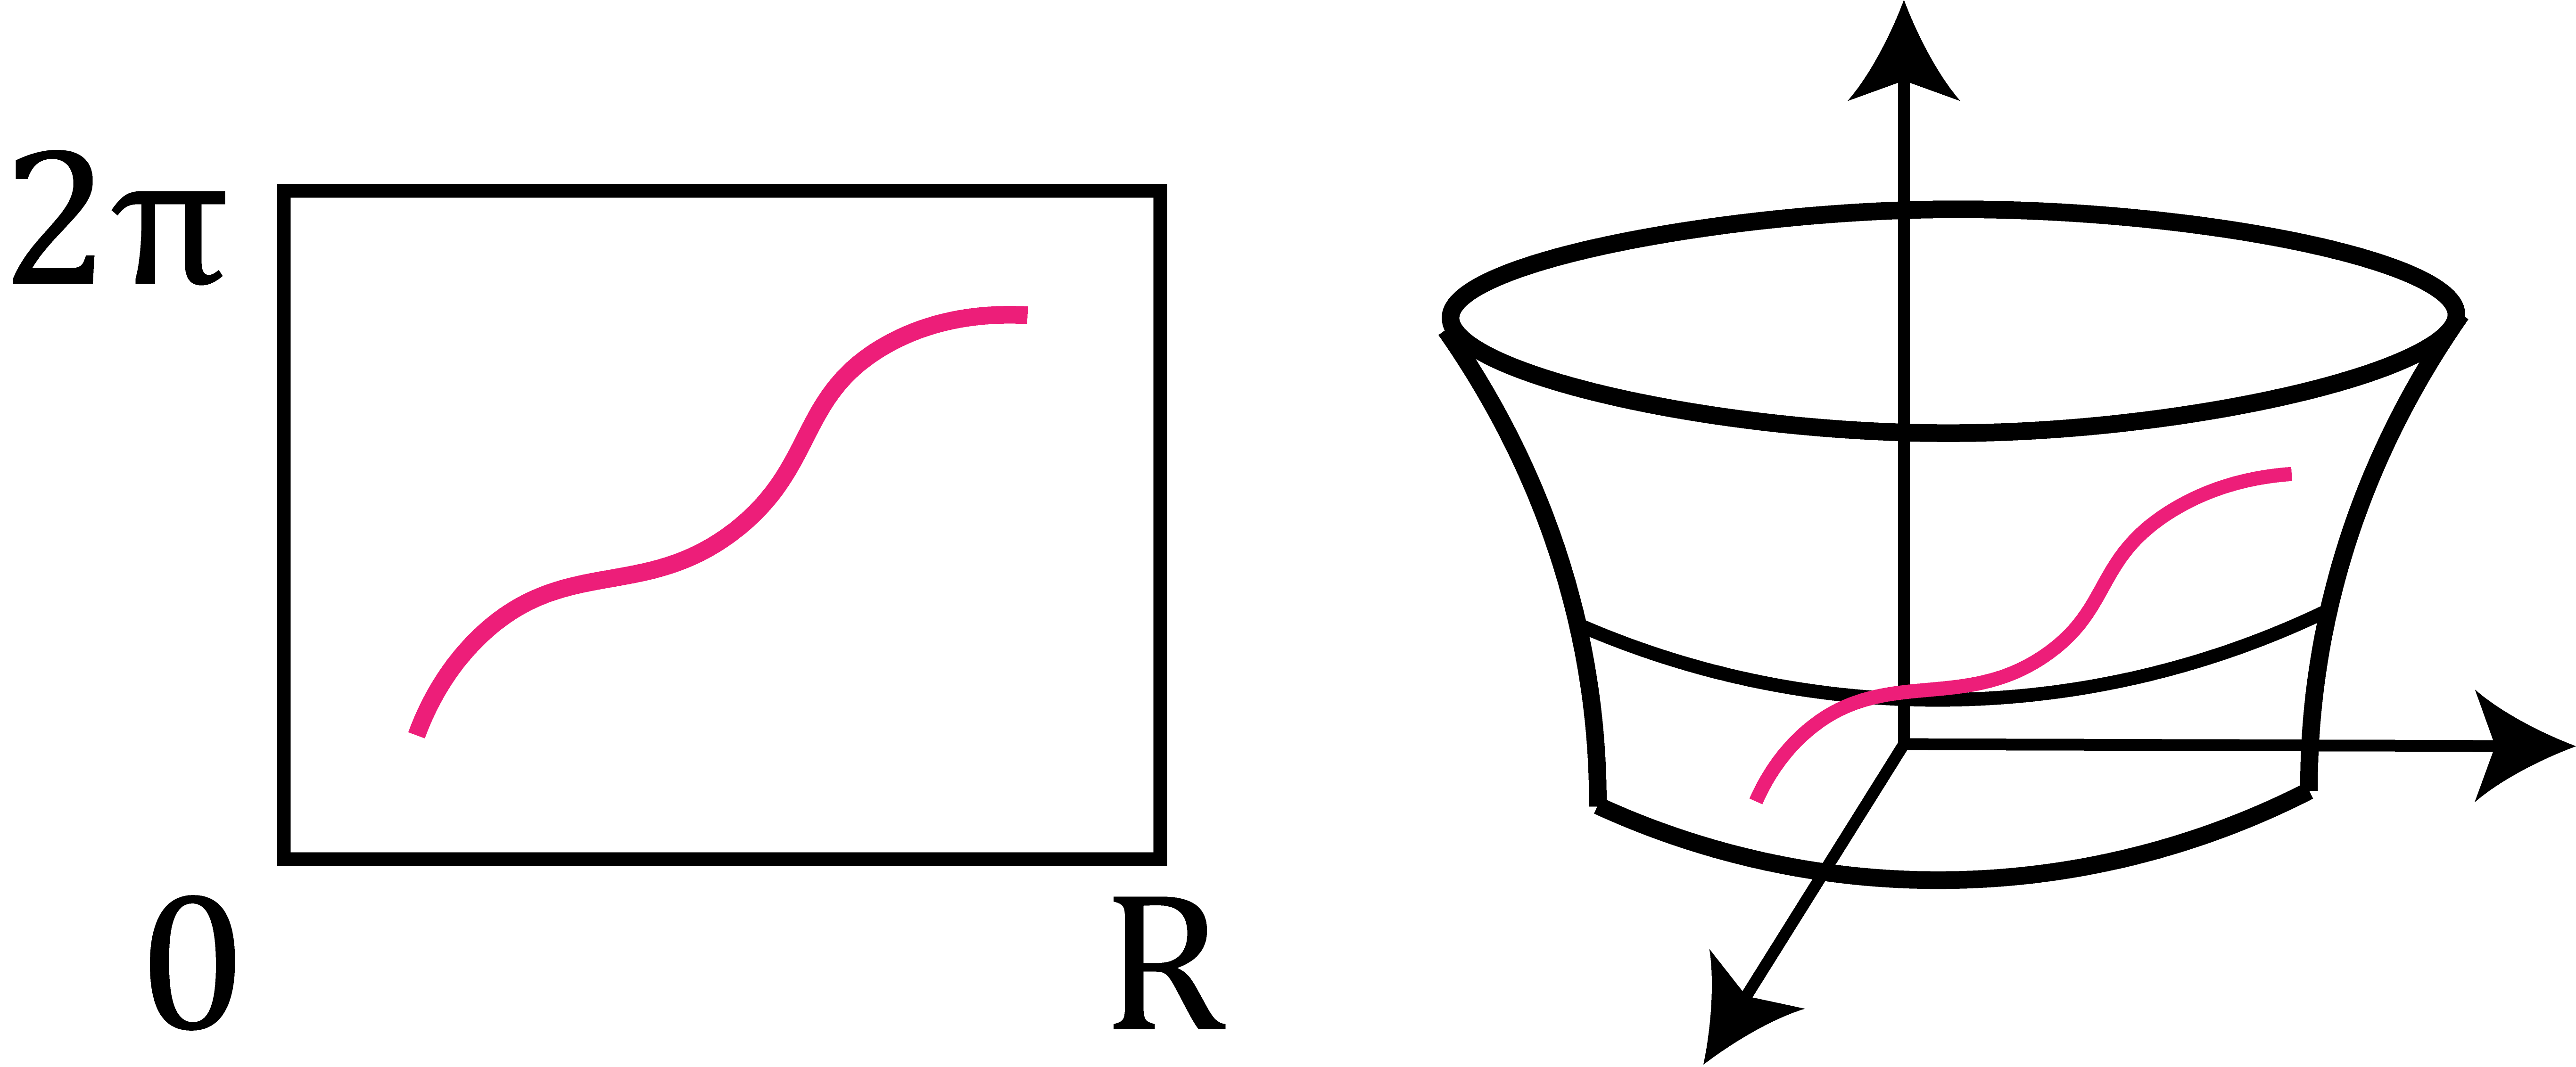
\includegraphics[width=6cm]{pics/15_1}
        \end{figure}
        \[\gamma(t) = (u(t),\ v(t)) \mapsto \int_0^1 |\dot{\Phi \times \gamma}| dt = \int_0^1 <\begin{pamtrix}
          \dot{u}\\
          \dot{v}
        \end{pamtrix},\ \RNumb{1}>\begin{pamtrix}
          \dot{u}\\
          \dot{v}
        \end{pamtrix} = \int_0^1 \sqrt{\dot{u}^2 + \Gamma^2(u(t)) \dot{v}^2} dt\]
        \[C^{\infty}([0,1],\ \R \times (0,\ 2\pi)) \ra \R\]
        \[\gamma(t) = (u(t),\ v(t)) \mapsto \us{L(u,v,\dot{u},\dot{v},t)}{\int_0^1 \Br{\dot{u}^2 + \Gamma^2(u(t)) \dot{v}^2} dt}\]
        \[\begin{cases}
            \dfrac{d}{dt} \Br{\dfrac{\d L}{\d \dot{u}}} - \dfrac{\d L}{\d u} = 0\\ \\
            \dfrac{d}{dt} \Br{\dfrac{\d L}{\d \dot{v}}} - \dfrac{\d L}{\d v} = 0
        \end{cases}\]
        \[\dfrac{\d L}{\d u} = 2 \dot{v}^2 \Gamma_{(u)} \Gamma_{(u)}' \qq \dfrac{\d L}{\d v} = 0\]
        \[\dfrac{\d L}{\d u} = 2 \dot{u} \qq \dfrac{\d L}{\d \dot{v}} = 2 \dot{v} \Gamma^2(u)\]
        \[\begin{cases}
            \ddot{u} - \Gamma(u) \Gamma'(u) \dot{v}^2 = 0\\
            \ddot{v} + 2 \dfrac{\Gamma'(u)}{\Gamma(u)} \dot{u} \dot{v} = 0
        \end{cases}\]
        \[\dfrac{d}{dt}\dfrac{\d L}{\d \dot{u}} = 2 \ddot{u}\]
        \[\dfrac{d}{dt}\dfrac{\d L}{\d \dot{v}} = 2 \Br{\ddot{v} \Gamma^2(\dot{u}) + 2\dot{v} r r' \dot{u}}\]
        \[\begin{cases}
            \dfrac{d}{dt} \Br{\dfrac{\d L}{\d \dot{u}}} - \dfrac{\d L}{\d u} = 0\\ \\
            \dfrac{d}{dt} \Br{\dfrac{\d L}{\d \dot{v}}} - \dfrac{\d L}{\d v} = 0
        \end{cases}\]
        Совпало
        \[\dot{v} r^2 (u) = C\]
        \[C = 0\]
        \[\dot{V} = 0 \RA V = \const\]
        \[\begin{cases}
            u = \alpha t + \beta\\
            v = \const
        \end{cases}\]
        \begin{figure}[H]
            \centering
            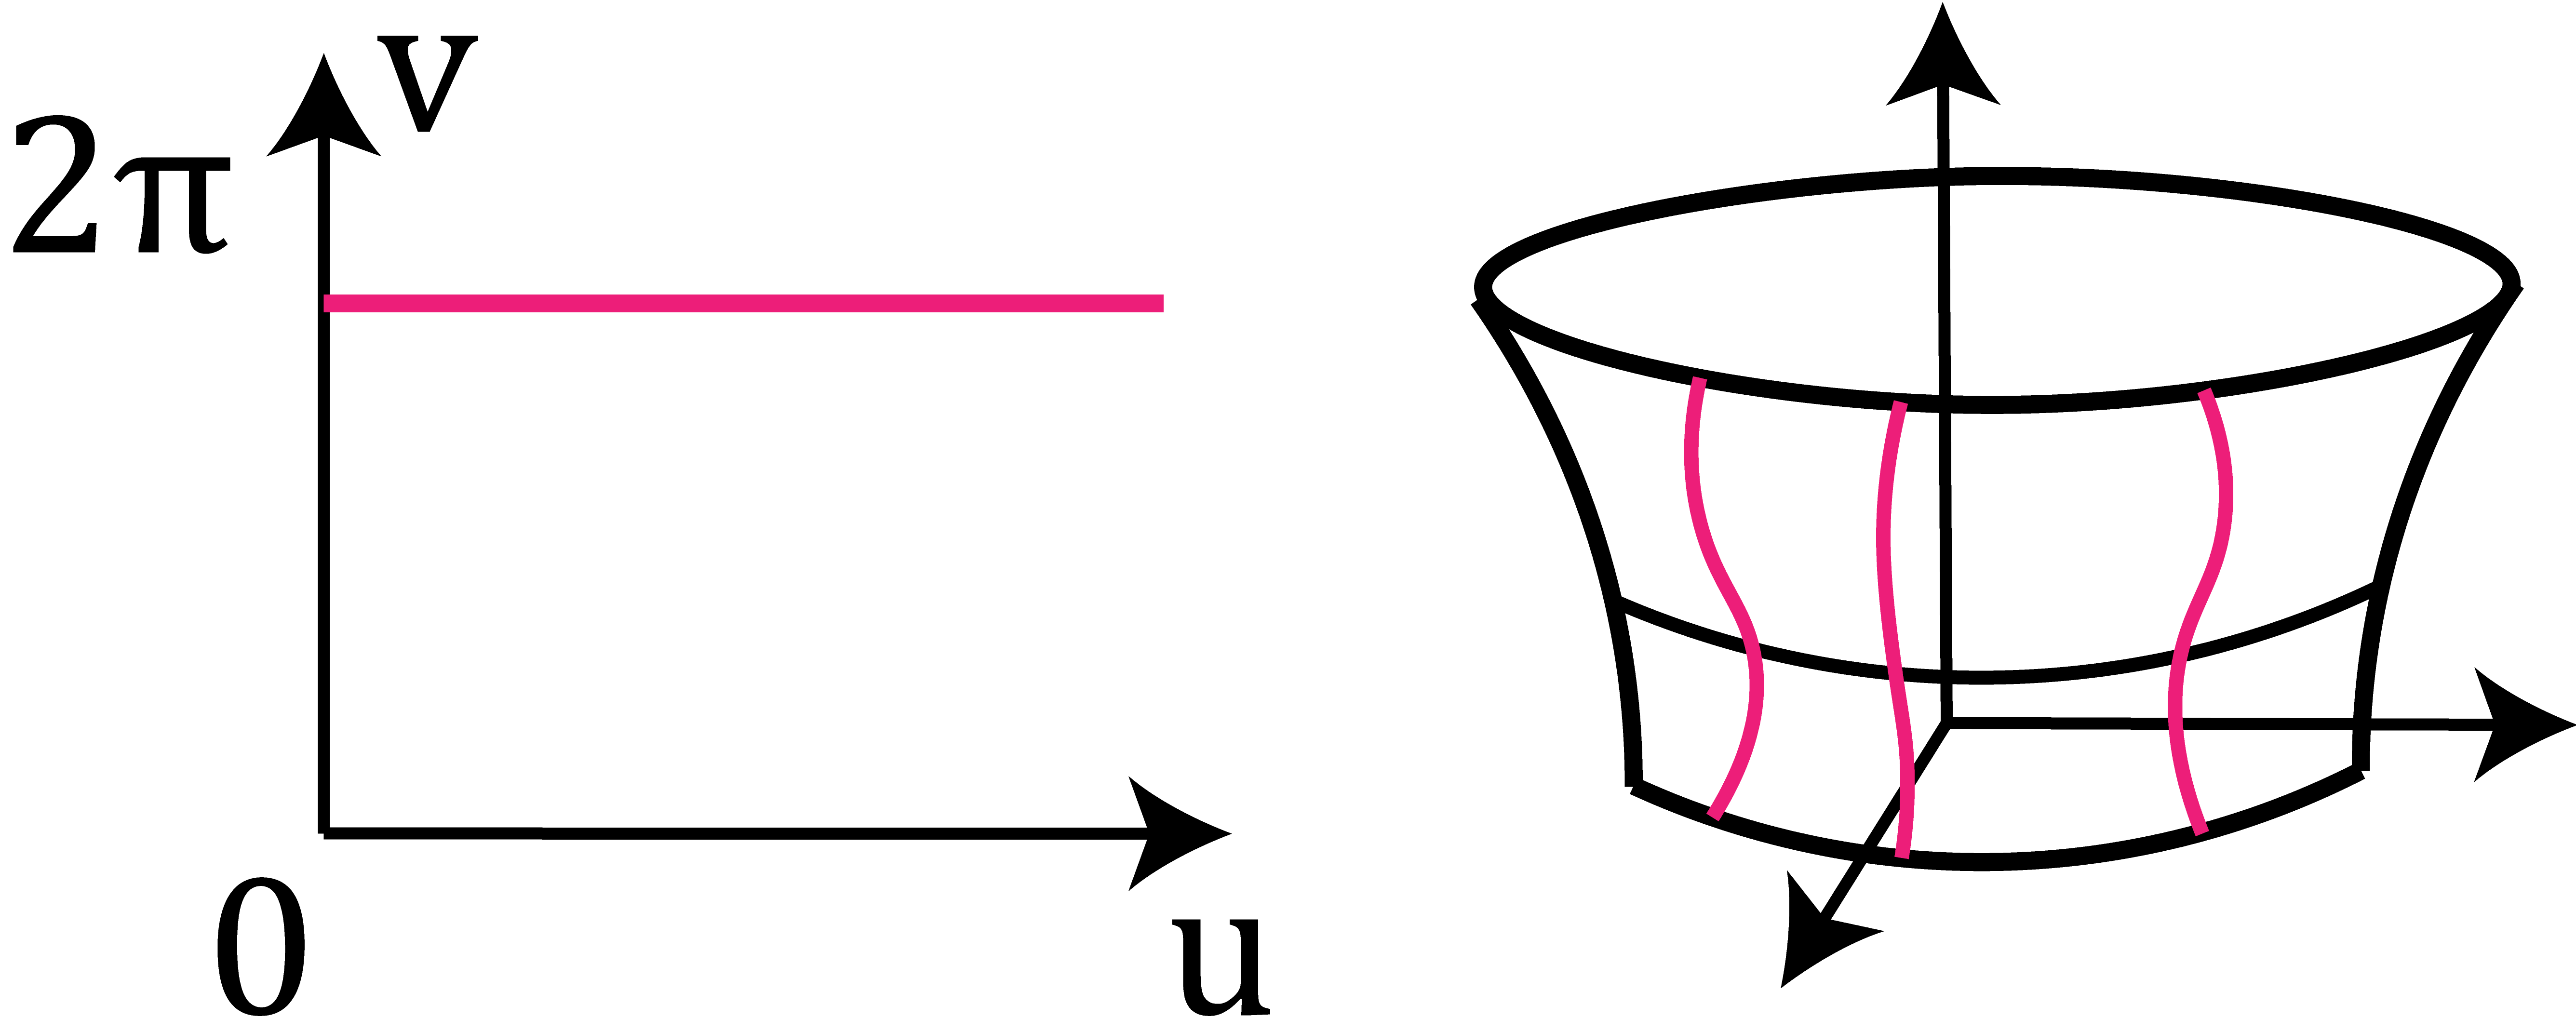
\includegraphics[width=6cm]{pics/15_2}
        \end{figure}
    \end{Sol}
\end{document}
